\chapter{Introduction}
\label{cpt:format}

% small blurb summary

\section{APT Background}

The Advanced Particle-astrophysics telescope is designed to be a successor to the Fermi Gamma-ray Space Telescope, which has surpassed its expected mission time of 10 years. The main objectives of the APT include studying high-energy transient phenomena such as supernovae or gamma-ray bursts (GRBs), continuing the search for dark matter, and conducting broader surveys of the sky in gamma rays. The APT would improve telescope sensitivity while maintaining a similar budget to the Fermi mission, allowing for a more extensive search for dark matter and an increased ability to detect high-energy transients.

\section{APT Design}

The APT is designed to be used in the mid-keV to low TeV energy range, which is a significant improvement on Fermi's detecting range. The final telescope will consist of 20 repeated layers of detecting material, spaced 15 cm apart, in a cube 3 meters tall and 2.5 meters on each side. The middle section of each layer - the calorimeter - records the energy of each photon or particle that interacts with it, and the WLS fibers on the top and bottom of each layer record the corresponding position of each interaction. From these detected interactions, we are able to reconstruct the initial direction of the photon source using software.

\begin{figure}
    \centering
    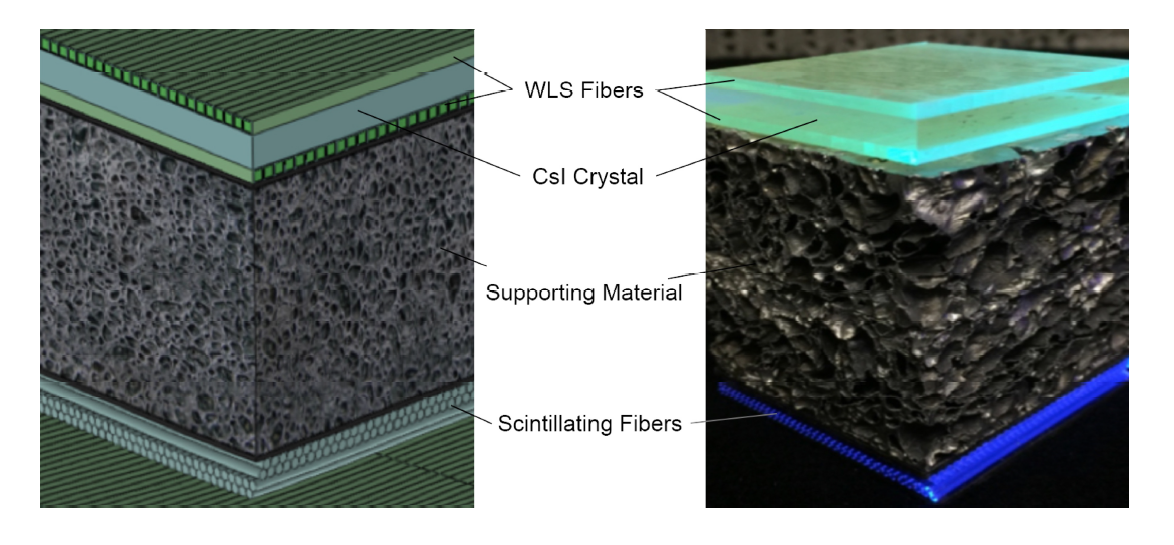
\includegraphics[width=0.7\textwidth]{APT_layers.png}
    \caption{One layer of the APT, shown as a computer model on the left and as a real-world prototype on the right, with aluminum used for the support structure. The Cesium Iodide (CsI) detects photon energy while the WLS fibers detect photon position. The scintillating fibers detect the position of any matter particles that enter the detector. Each subsequent layer would have the same structure as the one shown. \cite{APTmemo}}
    \label{fig:APT_layer}
\end{figure}

\section{APT Software}
The APT achieves such a broad energy range by using two different software methods for reconstructing the trajectories of incoming photons, one for each of the two dominant gamma-ray interactions in this energy range. Below approximately 30 MeV, the dominant interaction is called Compton scattering, a process by which a photon transfers some of its momentum to an electron, changing its resulting wavelength and trajectory. In the mid-MeV to GeV range, photons most commonly undergo a process called pair production upon entering the detector. As this research focuses on reconstructing Compton scatters, a thorough discussion of pair production is outside the scope of this paper, but more information can be found in almost any particle physics textbook or online.

\section{Gamma-ray Bursts}
A gamma-ray burst (GRB) is an extremely bright burst of gamma-rays from a point source in the sky. They were first discovered in the 1960s by a US satellite that had been set up to search for signs of nuclear blasts. The Compton Gamma-Ray Observatory (CGRO) was used to determine that GRBs originate mainly from outside the Milky Way. A GRB can last anywhere from a few milliseconds to several hours, which is an incredibly short time window compared to most other astronomical observations. Many astrophysicists now believe that short-duration GRBs are caused by neutron-star mergers, or collisions of extremely dense stellar remnants, while long-duration GRBs come from core-collapse supernovae, or explosions of high mass stars.

\iffalse
- extremely bright bursts of gamma-rays from point sources in the sky, lasting anywhere from several milliseconds to several hours, an incredibly short time compared to most phenomena studied in astronomy
- they leave afterglows after the initial burst, radiation which tails off gradually, but to our knowledge they never come from the same source twice
- short-duration GRBs are thought to be produced by neutron star mergers
    - extremely dense remnants of stars collide
- long-duration gamma-ray bursts are thought to be core-collapse supernovae, which occurs at the death of very massive stars, much greater than the mass of our sun
- their emission mechanisms are not yet well understood, the energies required indicate that the efficiency of matter to energy conversion is extremely high in these events
- they are recognizable by their light curves, though these light curves have a huge variation
- if we are able to detect a longer-duration GRB in its initial stages, we can signal its location to other observatories and get data not just at high wavelengths, but from optical or radio telescopes as well
- this will help us to better understand the causes of gamma-ray bursts, which could lead to lots of interesting astrophysics discoveries in the future
\fi

\section{Project Motivation}
Though several theories exist as to their causes, the emission mechanisms of GRBs are not yet well-understood. The energies involved indicate a very efficient conversion of matter to energy, and exactly how this occurs is still an open question in the field of astrophysics. To better understand the processes that produce GRBs, it would be highly useful to observe them simultaneously with multiple different telescopes at multiple different wavelengths (gamma-ray, optical, infrared, etc.) To do this, we must be able to search for and detect a GRB in its initial stages and send out its location to other observatories. Achieving this goal could lead to future discovery in the field of astrophysics as GRBs become better understood.

One major goal of the APT is to process gamma-ray events quickly enough to localize a source within a few seconds of the start of the burst and signal its location in that time. This means that we must significantly increase the detection capabilities of the APT in the low-energy range (10 keV - 10 MeV) such that the incoming photons' directions can be reconstructed as quickly as they are received by the detector. As Compton scattering is the dominant interaction at these low energies, the primary focus of this research is to develop and test an algorithm to reconstruct Compton-scattered photons quickly and accurately enough that the telescope can pinpoint their source in close to real time. Many Compton telescopes rely on photon events with only two interactions to reconstruct their source positions. However, a significant fraction of events in the 0.5 - 10 MeV range will scatter twice or more in the detector, which means that we can achieve significant performance improvement by incorporating the reconstruction of multi-scatter events into our algorithm.

\section{Scientific Constraints}

To eventually reach the main goal of this project, several factors be taken into account at this stage. The telescope must be able to reconstruct the trajectories of gamma rays at or near the speed at which they enter the detector, with low latency between the initial detection and the reconstructed solution. During a gamma-ray burst, we expect to see [x]* photons per second, so our goal for reconstruction speed is approximately 50,000 photons per second, with a latency of 1 second or less. The telescope must also be able to reconstruct photons as accurately as possible given the time constraints. We believe that a 75\% accuracy level or above will allow us to successfully resolve a gamma-ray burst within two seconds or less. One of our other concerns is power consumption - the telescope will be part of a larger scientific instrument with a fixed amount of energy available to it daily. As such, we estimate that it cannot use more than 50 watts of power when running the reconstruction software.

\section{Process}
Using an algorithm found in \emph{Boggs \& Jean (2000)}\cite{Boggs} as a basis, we were able to write a Compton reconstruction algorithm that meets our goals for this project. We started with a sequential algorithm, trying each possible ordering of hits, and improved its performance by incorporating a tree search and several other methods to improve the runtime. We built a simple gamma ray simulator for our development and initial tests of reconstruction speed and accuracy. We found that the improved algorithm was able to reconstruct tens of thousands of photons per second with 80-90\% accuracy, which we believe will be enough to detect and localize a gamma-ray burst once the telescope is operational. By varying parameters in the algorithm, we also examine trends in the speed and accuracy, and discuss some possible trade-offs between the two.

\section{Related Work}
One of the best papers available on Compton reconstruction procedures is \emph{Boggs \& Jean} (2000)\cite{Boggs} which details the mathematical formulae and steps required to reconstruct the initial direction of a Compton event in a layered detector. Though the paper focuses more on the physics of reconstructing Compton scatters than the algorithmic parameters, the equations listed served as a very helpful starting point for building and refining our code. We developed with the purpose of creating an algorithm to be as fast and lightweight as possible while still meeting our accuracy requirements. Many Compton telescopes must transfer data over a network connection or save observations in order to reconstruct them later, but our program is designed to process data in real time, before it leaves the telescope.

\iffalse
- Boggs \& Jean
        - focused more on the physics than the CS
        - Gives us a basic algorithm to improve upon
- Zoglauer's Megalib
- COMPTEL
    - It uses Compton scattering to detect GRBs, like our detector
    - But it only has two layers (lower probability of interaction) and as such it can only detect two-scatter events, a small fraction.
    - Has a good signal-to-noise ratio, which may be harder to emulate with the APT as it has a much larger detecting area
    - Might be more easy to determine polarization with more layers - Compton scattering is sensitive to photon polarization, so more Compton scatters would give us more chances to determine if the scattering angles have a preferential direction \cite{COMPTEL}.
    - It also has a Time Of Flight detector, which our telescope lacks
    - They also used Geant for testing
- COSI
    - It is also a multiple compton scattering detector
    - flies up on a balloon instead of being space-based
- MEGALib
    - basically the exact same thing as our algorithm but better
    - Realta package can reconstruct Compton events in real time
    - As far as I can tell, the only difference is you need an internet connection
\fi